\usetikzlibrary{calc,arrows.meta,patterns,angles,quotes}
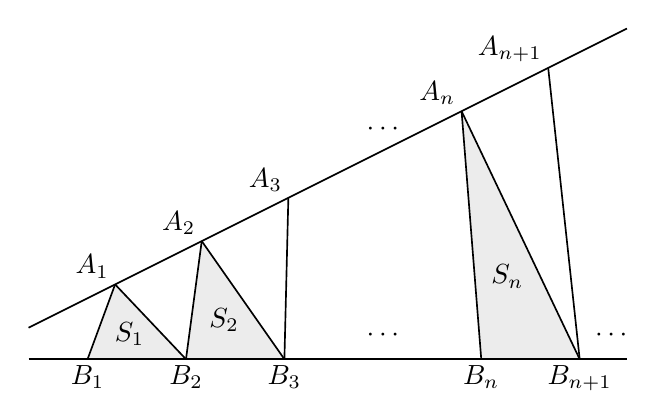
\begin{tikzpicture}[x=1cm,y=1cm,line width=.6pt,font=\normalsize,>=Stealth]
\coordinate (A1) at (0.9000000000,0.9500000000);
\coordinate (B1) at (0.5500000000,0.0000000000);
\coordinate (A2) at (2.0000000000,1.5000000000);
\coordinate (B2) at (1.8000000000,0.0000000000);
\coordinate (A3) at (3.1000000000,2.0500000000);
\coordinate (B3) at (3.0500000000,0.0000000000);
\coordinate (An) at (5.3000000000,3.1500000000);
\coordinate (Bn) at (5.5500000000,0.0000000000);
\coordinate (An1) at (6.4000000000,3.7000000000);
\coordinate (Bn1) at (6.8000000000,0.0000000000);
\fill[gray!15] (A1)--(B1)--(B2)--cycle;
\fill[gray!15] (A2)--(B2)--(B3)--cycle;
\fill[gray!15] (An)--(Bn)--(Bn1)--cycle;
\draw (-.2,.4)--(7.4,4.2);\draw (-.2,0)--(7.4,0);
\draw (A1)--(B1);
\draw (A1)--(B2);
\draw (A2)--(B2);
\draw (A2)--(B3);
\draw (An)--(Bn);
\draw (An)--(Bn1);
\draw (A3)--(B3);
\draw (An1)--(Bn1);
\node[above left=2pt,inner sep=0pt] at (A1) {$A_1$};
\node[below=2pt,inner sep=0pt] at (B1) {$B_1$};
\node[above left=2pt,inner sep=0pt] at (A2) {$A_2$};
\node[below=2pt,inner sep=0pt] at (B2) {$B_2$};
\node[above left=2pt,inner sep=0pt] at (A3) {$A_3$};
\node[below=2pt,inner sep=0pt] at (B3) {$B_3$};
\node[above left=2pt,inner sep=0pt] at (An) {$A_n$};
\node[below=2pt,inner sep=0pt] at (Bn) {$B_n$};
\node[above left=2pt,inner sep=0pt] at (An1) {$A_{n+1}$};
\node[below=2pt,inner sep=0pt] at (Bn1) {$B_{n+1}$};
\node at (1.0833333333,0.3166666667) {$S_1$};
\node at (2.2833333333,0.5000000000) {$S_2$};
\node at (5.8833333333,1.0500000000) {$S_n$};
\node at (4.3000000000,2.9200000000) {$\cdots$};
\node at (4.3000000000,0.3000000000) {$\cdots$};
\node at (7.2000000000,0.3000000000) {$\cdots$};
\end{tikzpicture}
